\documentclass{article}

\usepackage[english,french]{babel}
\usepackage[utf8]{inputenc}
\usepackage[T1]{fontenc}
\usepackage{amsmath, amsfonts, amssymb, amsthm}
\usepackage{bbm,algorithmic,algorithm,verbatim}

\usepackage{color}
\usepackage{subcaption}
\usepackage[pdftex]{graphicx}
\usepackage{epsfig}
\usepackage{ulem, stmaryrd, dsfont}
\usepackage{hyperref}

% the following were missing:

\usepackage{./tex/scribe}
\usepackage{./tex/shortcuts_js}

%%%%%%%%%%%%%%%%%%%%%%%%%%%%%%%%%%%%%%%%%%%%%%%%%%%%%%%%%%%%%%%%%%%%%%%%%%%%%%%
% Hyperlinks
%%%%%%%%%%%%%%%%%%%%%%%%%%%%%%%%%%%%%%%%%%%%%%%%%%%%%%%%%%%%%%%%%%%%%%%%%%%%%%%

\PassOptionsToPackage{hyphens}{url}
%\usepackage[pdftex,linkcolor=test,citecolor=vsomb_col,
%colorlinks=true,pagebackref,bookmarks=true,plainpages=true,
%urlcolor=fb_col]{hyperref}
\usepackage{cleveref}

%%%%%%%%%%%%%%%%%%%%%%%%%%%%%%%%%%%%%%%%%%%%%%%%%%%%%%%%%%%%%%%%%%%%%%%%%%%%%%%
%%%%%%%%%%%%%%%%%%%%%%%%%%%%%%%%%%%%%%%%%%%%%%%%%%%%%%%%%%%%%%%%%%%%%%%%%%%%%%%

\begin{document}
\sloppy
\lecture{HMMA308}{Large Dimension Probabilistic Methods}{Ali Rahimi and Ben Recht}{Cassandre Lepercque}


\section{Introduction}
Because of the growing size of data, usual techniques of linear algebra need to be revisited in large-dimension models. To answer that, we use more and more probabilistic and statistical methods, like: sub-sampling, random projections, etc. The most important stakes are based on the improvement of techniques like SVD (\textit{Singular Value Decomposition}) and PCA (\textit{Principal Component Analysis}). \\
It is a multi-faced challenge, because lots of scientist work have the same problem: data are growing in an exponential way.  For example, a dataset with half a million training examples might take days to train on modern workstations.\\
To accelerate the training of kernel machines, we propose to map the input data to a randomized low-dimensional feature space and then apply existing fast linear methods. \\

Kernel machines such as the Support Vector Machine are attractive because they can approximate any function or decision boundary arbitrarily well with enough training data. But, the methods that work on the data kernel matrix are ill-suited to the size of the training dataset. On the other hand, in the "linear" framework of SVMs, algorithms and regularized regression run much faster when the dimension of the data is small because they operate on the covariance matrix rather than on the kernel matrix of the training data. We are going to proposed a way to combine the advantages of the linear and nonlinear approaches. We know that, random features significantly reduce the computation needed for training, and obtain similar or better testing error, because if we combine them with simple linear learning techniques, we get pretty much the same as with advanced classification and regression algorithms.

\section{The mathematical approach}

We are going to use features for algorithms that depend only on the inner product between pairs of input points. It is based on  the observation that any positive definite function $k(x,y)$ with $x,y\in \bbR^d$ defines an inner product and a lifting $\phi$ so that the inner product between lifted datapoints can be quickly computed as
\begin{equation*}
    \langle \phi(x), \phi(y)\rangle = k(x,y).
\end{equation*}
And we know that the cost is that algorithms access the data only through evaluations of $k(x,y)$, or through the kernel matrix,  consisting of $k$ applied to all pairs of datapoints. As a result, large training sets incur large computational and storage costs. But the conclusion from this is that large training sets have a high computational and storage cost.

We are going to propose explicitly mapping the data to a low-dimensional Euclidean inner product space using a randomized feature map $z: \bbR^d \rightarrow \bbR^D$ instead of doing it on the implicit lifting that we saw above.
\newpage
We are doing this mapping so that the inner product between a pair of transformed points approximates their kernel evaluation:
\begin{equation*}
    k(x, y) = \langle \phi(x), \phi(y) \rangle \approx z(x)' z(y),
\end{equation*}
where, $z'$ is the transposed matrix of $z$ and $z$ is low-dimensional. \\
We can transform the input with $z$ and apply fast linear learning methods to approximate the result of the corresponding non-linear kernel machine. \\

We are now, going to show how to construct feature spaces that uniformly approximate popular shift-invariant kernels $k(x-y)$ in $\epsilon$ with only $D = O(d \epsilon^{-2} \times log (\epsilon^{-2}))$ dimensions, and empirically show that great classification and regression performance can be obtained for even smaller $D$. 
So, these randomized feature maps gives us access to extremely fast learning algorithms but they also provide a way to quickly evaluate the machine. To evaluate the machine at a test point $x$ we need to computing
\begin{equation*}
    f(x) = \sum_{i=1}^N c_i \ k(x_i, x),
\end{equation*}
which requires $O(N\times d)$ operations to compute and retraining much of the dataset unless the machine is very sparse. Usually, this is unacceptable for large datasets. \\

From another side, after learning a hyperplane $w$, a linear machine can be evaluated by simply computing, 
\begin{equation*}
    f(x) = w' \times z(x),
\end{equation*}
which requires (with the randomized feature maps) only $O(D+d)$ operations and storage. \\
Our goal, is to demonstrate two randomized feature maps for approximating shift invariant kernels.\\

In the next two sub-parts, we are going to see the first randomized maps that consists of sinusoids randomly drawn from the Fourier transform of the kernel function we want to approximate, and because this map is smooth, ti is well-suited for interpolation tasks. \\
The second randomized map partitions the input space using randomly shifted grids at randomly choser resolutions but, unlike the first randomized map, this mapping is not smooth. But, leverages the proximity between input points ans is well-suited for approximating kernels that depend on the $L_1$ distance between datapoints. \\
The randomized maps are given by, 
\begin{itemize}
    \item Random Fourier Features
    \item Random Binning Features 
\end{itemize}

\subsection{Random Fourier Features}

Our first set of random features consists of random Fourier bases $cos(\omega' x + b)$ where,
\begin{itemize}
    \item $\omega \in \bbR^d$, 
    \item  $b \in \bbR$,
\end{itemize}
are random variables. \\
Those maps project data points on a randomly chosen line and pass the resulting scalar through a sinusoidal function (as we can see in Figure \ref{Projection_data_points}). 
\begin{figure}[h!]
    \centering
    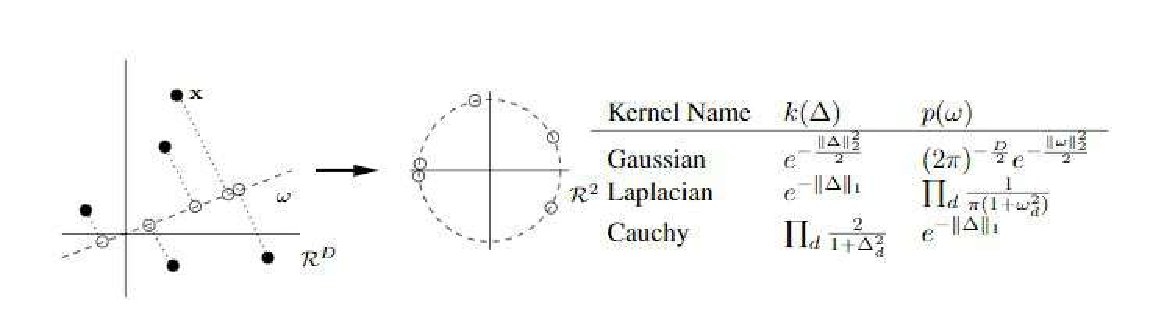
\includegraphics[scale=0.7]{images/Random_fourier_features.pdf}
    \caption{Each component of the feature map $z(x)$ projects $x$ onto a random direction $\omega$ drawn from the Fourier transform $p(\omega)$ of $k(\Delta)$, and wraps this line onto the unit circle in $\bbR^2$.}
    \label{Projection_data_points}
\end{figure}

By doing this, we can see that the direction of these lines from an appropriate distribution guarantees that the product of two transformed points will approximate a desired shift-invariant kernel.\\

We are now, going to see, a theorem from harmonic analysis.
\begin{theorem}(Bochner)\\
A continuous kernel $k(x,y) = k(x - y)$ on $\bbR^d$ is positive definite if and only if $k(\delta)$ is the Fourier transform of a non-negative measure.
\end{theorem}

If a shift-invariant kernel $k(\delta)$ is properly scaled, Bochner’s theorem guarantees that its Fourier transform $p(\omega)$ is a proper probability distribution. It is define by $\zeta_{\omega}(x) = e^{j\omega'x}$, and we have, 
\begin{equation}
        k(x-y) = \int_{\bbR^d} p(\omega) \times e^{j\omega'(x-y)}d\omega \\
        = \bbE_{\omega}[\zeta_{\omega}(x) \ \zeta_{\omega}(y)\*],
\end{equation}
so, $\zeta_{\omega}(x) \ \zeta_{\omega}(y)\*$ is an unbiased estimate of $k(x,y)$ when $\omega$ is drawn from $p$.\\
If both of the probability distribution $p(\omega)$ and the kernel $k(\delta)$ are real, the integral we just saw, converges when the exponential (complex) are replaced with cosines. Thus, we may obtain a real-valued mapping that satisfies the $\bbE[z_{\omega}(x)\ z_{\omega}(y)] = k(x,y)$ condition by setting $z_{\omega}(x)$ as $\sqrt{2} cos(\omega' x + b)$, where
\begin{itemize}
    \item $\omega$ is drawn from $p(\omega)$,
    \item $b$ is drawn uniformly from $[0, 2\pi]$.
\end{itemize}

We can lower the variance of the estimate of the kernel by concatenating $D$ randomly chosen $z_{\omega}$ into one D-dimensional vector $z$ and normalizing each component by $\sqrt{D}$. The inner product
\begin{equation*}
   z(x)' z(y) = \frac{1}{D} \sum_{j=1}^D z_{\omega_j}(x) z_{\omega_j}(y)  
\end{equation*}
is a sample average of $z_{\omega}$ and is a lower variance approximation to the expectation (1).\\

While $z_{\omega}$ is bounded between $+ \sqrt{2}$ and $-\sqrt{2}$ for a fixed pair if points $x$ and $y$, \textit{Hoeffding}'s inequality guarantees exponentially fast convergence in $D$ between $z(x)' z(y)$ and $k(x,y): \Pr [|z(x)' z(y) - k(x,y)| \geq \epsilon] \leq 2\times e^{-\frac{D\epsilon^2}{4}}$. By this observation, we can have a much stronger assertion, which can be proven for every pair of points in the input space simultaneously, 

\newpage
\begin{remark}(Uniform convergence of Fourier features)\\
Let $\mathcal{M}$ be a compact subset of $\bbR^d$ with diameter $\diam(\mathcal{M})$. Then, for the mapping $z$, we have
\begin{equation*}
    \Pr \left[\sup_{x,y \in \mathcal{M}} |z(x)'z(y)-k(x,y)| \geq \epsilon \right] \leq 2^8 \left( \frac{\sigma_p \diam(\mathcal{M})}{\epsilon} \right)^2 e^{-\frac{D\epsilon^2}{4(d+2)}}, 
\end{equation*}
where $\sigma_p^2 \equiv \bbE_p[\omega' \omega]$ is the second moment of the Fourier transform of $k$.\\
Furthermore, 
\begin{equation*}
    \sup_{x,y \in \mathcal{M}} |z(x)'z(y)-k(x,y)| \leq \epsilon
\end{equation*}
with any constant probability when $D = \Omega\left( \frac{d}{\epsilon^2} log(\frac{\sigma_p \diam(\mathcal{M})}{\epsilon}) \right)$.
\end{remark}

The proof of this assertion first guarantees that $z(x)'z(y)$ is close to $k(x-y)$ for the centers of an $\epsilon$-net over $\mathcal{M} \times \mathcal{M}$. This result is then extended to the entire space using the fact that the feature map is smooth with high probability. \\
By a standard Fourier identity, the scalar $\sigma_p^2$ is equal to the trace of the Hessian of $k$ at 0.  It quantifies the curvature of the kernel at the origin. For the spherical Gaussian kernel, $k(x,y) = e^{(-\gamma \| x-y \| ^2)}$, we have $\sigma_p^2 = 2d\gamma$.


\subsection{Random Binning Features}
Our second random map partitions the input space. It is using randomly shifted grids at randomly chosen resolutions and assigns to an input point a binary bit string that corresponds to the bins in which it falls (as you can see in Figure \ref{Random_shift_grids}).
\begin{figure}[h!]
    \centering
    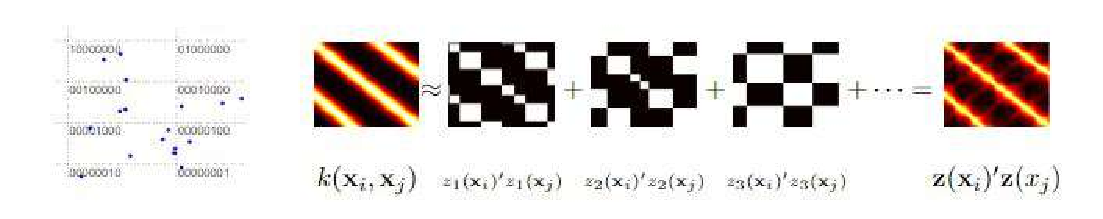
\includegraphics[scale=0.7]{images/Radom_binning_features.pdf}
    \caption{On the \textit{left} side, you can see what the algorithm does. It repeatedly partitions the input space using a randomly shifted grid at a randomly chosen resolution and assigns to each point $x$ the bit string $z(x)$ associated with the bin to which it is assigned. On the \textit{right} side, you can see the binary adjacency matrix that describes this partitioning has $z(x_i)'z(x_j)$ in its $ij$-th entry and is an unbiased estimate of kernel matrix.}
    \label{Random_shift_grids}
\end{figure}

We know that it uses rectilinear grids consequently, this mapping is well-suited for kernels that depend only on the $L_1$ distance between pairs of points.\\
We build the grids in that way so that the probability that two points $x$ and $y$ are assigned to the same bin is proportional to $k(x,y)$. \\
We have the inner product between a pair of transformed points is proportional to the number of times the two points are binned together and so that it is an unbiased estimate of $k(x,y)$.

\newpage
Let's explain how it goes. First we describe a randomized mapping to approximate the "hat" kernel as, 
\begin{equation*}
    \hat{k}(x,y; \delta) = \max \left(0,\ 1-\frac{|x-y|}{\delta} \right),
\end{equation*}
on a segment of $\bbR$, then we show how to build mappings for more general separable multi-dimensional kernels. Then we partition the real number line with a grid of pitch $\delta$ and we randomly shift this grid by an amount $u$ that we have drawn uniformly at random from $[0, \delta]$. It seems that this grid partitions the real number line into intervals $[u + n\delta, \ u + (n+1) \delta]$ for all integers $n$. Therefore, the probability that two points $x$ and $y$ fall in the same bin in this grid is $\max \left(0, \ 1-\frac{|x-y|}{\delta} \right)$.\\

Secondly, we consider shift-invariant kernels that can be written as a convex combinations of "hat" kernels on a compact subset of $\bbR \times \bbR : k(x,y) = \int_0^{\infty} \hat{k}(x,y;\delta)\ p(\delta) d\delta$. If the pitch $\delta$ of the grid is sampled from $p$, $z$ gives a random map again for $k$, because, 
\begin{equation*}
    \bbE_{\delta, u}[z(x)'z(y)] = \bbE_{\delta}[\bbE_u[z(x)'z(y) | \delta]] = \bbE_{\delta}[\hat{k}(x,y;\delta)] = k(x,y).
\end{equation*}
On other words, we have the probability that $x$ and $y$ are binned together equal $k(x,y)$ if the pitch $\delta$ of the grid is sampled from $p$ and the shift $u$ is drawn uniformly from $[0, \delta]$.\\

Random maps for separable multivariate shift-invariant kernels of the form $k(x-y) = \prod_{m=1}^d k_m (|x^m - y^m |)$ (like the multivariate Laplacian kernel) can be build in a similar way if each $k_m$ can be written as a convex combination of "hat" kernels. In the binning process above, we apply each dimension of $\bbR^d$ independently and we have the probability that $x^m$ and $y^m$ are binned together in dimension $m$ is $k_m(|x^m - y^m|)$. While the binning process is independent across dimensions, we have the probability that $x$ and $y$ are binned together in every dimension is $\prod_{m=1}^d k_m(|x^m - y^m|) = k(x,y)$. \\
It is in this multivariate case, that we have $z(x)$ which encodes the integer vector $[\hat{x}^1, \cdots, \hat{x}^d]$ corresponding to each bin of the $d$-dimensional grid as a binary indicator vector. \\
In the practice case, our implementation eliminates unoccupied bins from the representation when computing $z(x)$ when $d$ is large, and since there are never more bins than training points, this ensures no overflow is possible. \\

To reduce the variance of the estimator $z(x)' z(y)$, we can concatenating $P$ random binning functions $z$ into an larger list of features $z$ and scaling by $\sqrt{\frac{1}{P}}$. So we have the inner product, 
\begin{equation*}
    z(x)'z(y) = \frac{1}{P} \sum_{p=1}^P z_p(x)' z_p(y),
\end{equation*}
is the average of $P$ independent $z(x)' z(y)$ and has therefore lower variance.\\
While $z$ is binary, we have that \textit{Hoeffding}'s inequality guarantees that for a fixed pair of points $x$ and $y$, $z(x)'z(y)$ converges exponentially quickly to $k(x,y)$ as $P$ increases. We have the following remark which explain that this convergence holds simultaneously for all points.

\newpage
\begin{remark}
Let $\mathcal{M}$ be a compact subset of $\bbR^d$ with diameter $\diam(\mathcal{M})$. Let $\alpha = \bbE[\frac{1}{\delta}]$ and let $L_k$ denote the Lipschitz constant of $k$ with respect to the $L_1$ norm. With $z$ as above, we have 
\begin{equation*}
    \Pr \left[ \sup_{x,y \in \mathcal{M}} |z(x)'z(y) - k(x,y)| \leq \epsilon \right] \geq 1 - 36\ d \ P \ \alpha \ \diam(\mathcal{M}) exp\left( \frac{-\left( \frac{P\epsilon^2}{8} + ln(\frac{\epsilon}{L_k}) \right)}{d+1} \right).
\end{equation*}
Note, 
\begin{equation*}
    \alpha = \int_0^{\infty} \frac{1}{\delta} p(\delta) d\delta = 1,
\end{equation*}
where $L_k = 1$ for the Laplacian kernel. 
\end{remark}

The explanation of this remark is, while the function $z$ is piecewise constant over $\mathcal{M}$, $\mathcal{M} \times \mathcal{M}$ can be broken up into a few small rectangular cells so that throughout each cell, $k(x,y)$ does not change much and $z(x)$ and $z(y)$ do not change at all. \\
 With high probability, at the centers of these cells $z(x)'z(y)$ is close to $k(x,y)$, which guarantees that $k(x,y)$ and $z(x)'z(y)$ are close throughout $\mathcal{M}$.M


\section{Example part}
In this part, we will do a comparison of the previous methods on a dataset.\\
We use the dataset $load_digits(n_{class}=9)$ for the \textit{sklearn} python package. In Figure \ref{data_plot}, we can see how the dataset is settle. 

\begin{figure}[h!]
    \centering
    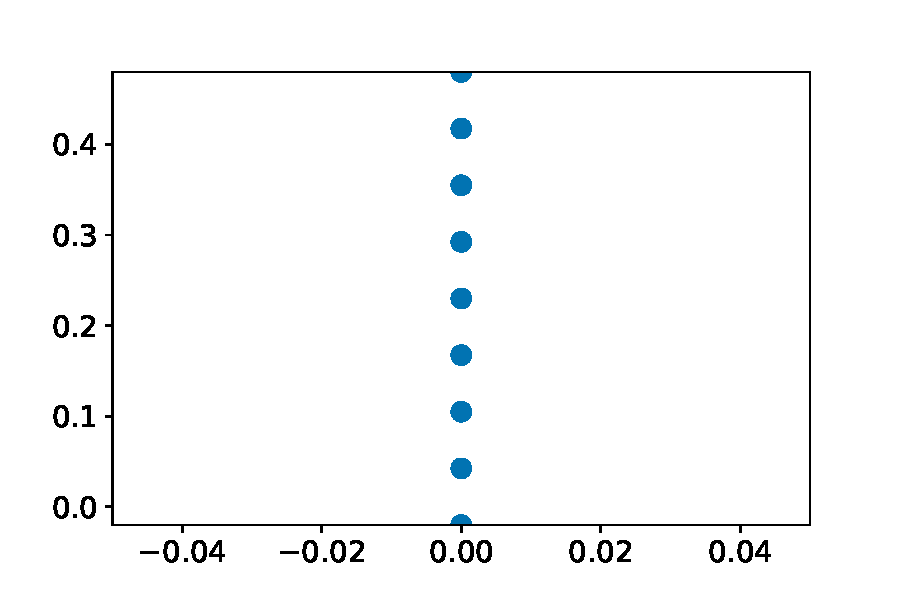
\includegraphics[scale=0.7]{images/plot_data.pdf}
    \caption{Visualization of the dataset.}
    \label{data_plot}
\end{figure}

First, we are going to see the random Fourier features against the SVM method. 
As we can see in the left side of the Figure \ref{accuracy_time}, the classification accuracy of the Fourier approximation grows from less than 0.8\% to approximately 0.95\%, which compares to other methods, is very good. Indeed, the linear SVM method is around 0.93\% while the radial basis function is around 0.97\%. 

\newpage
On the right side of Figure \ref{accuracy_time}, we see that the training times is growing (in the fast way) for the Fourier approximation. Step by step, it is going faster.  \\
\begin{figure}[h!]
    \centering
    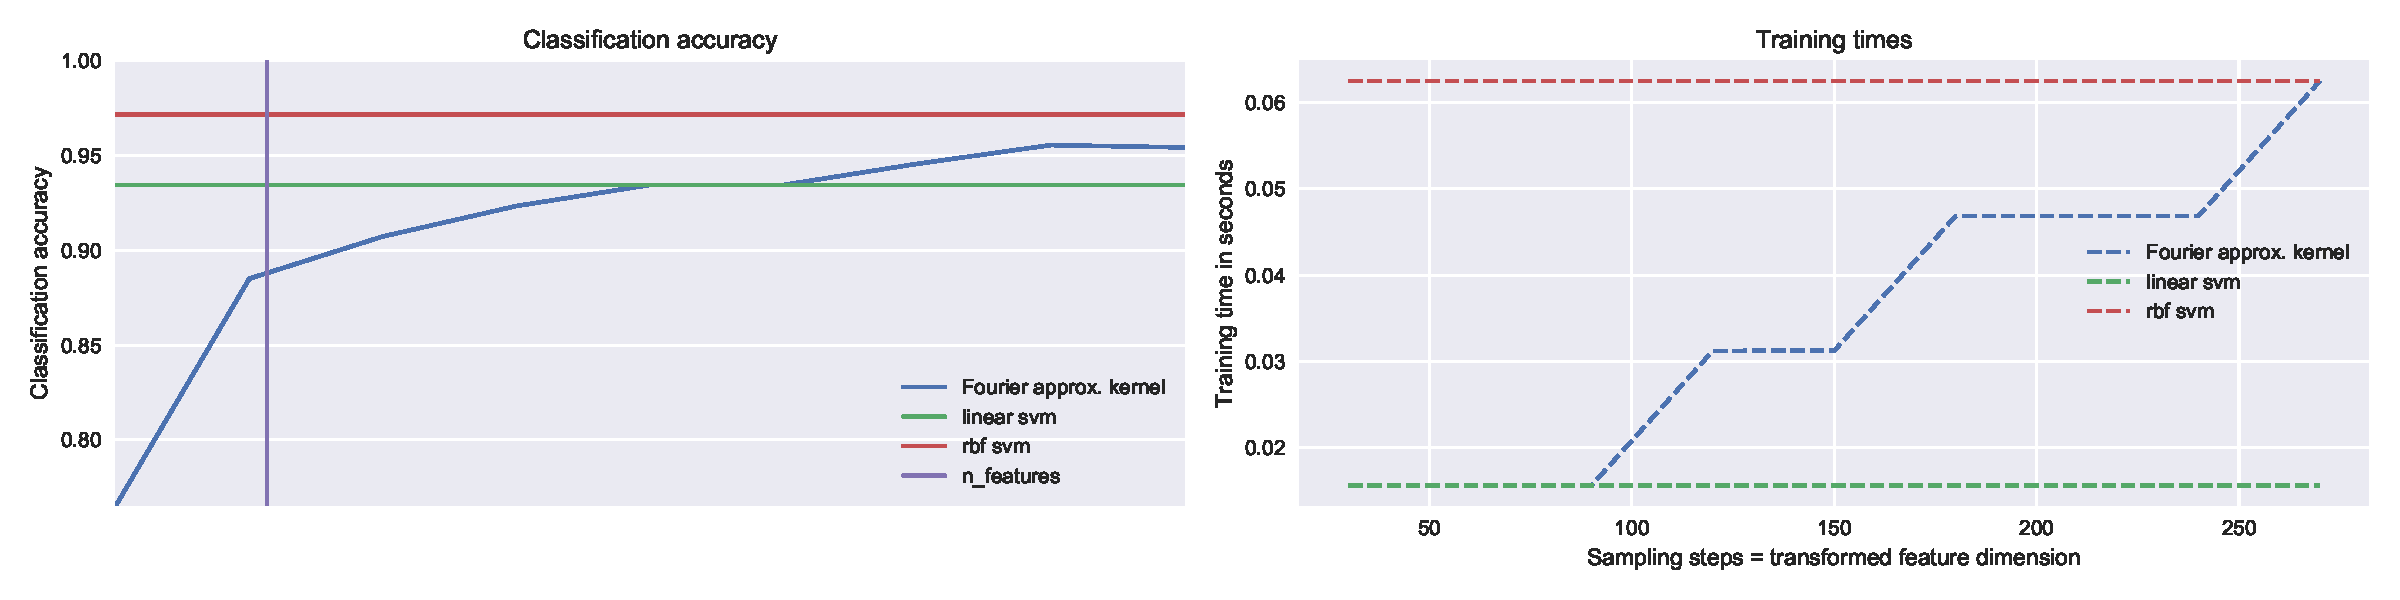
\includegraphics[scale=0.45]{images/accuracy_and_timescale.pdf}
    \caption{Classification accuracy (left) and Training times (right) of the dataset.}
    \label{accuracy_time}
\end{figure}

Let's take a closer look to the score of theses methods. 
\begin{table}[h!]
   \centering
    \begin{tabular}{|p{2cm}||p{3cm}|p{3cm}|p{3cm}|}
    \hline
    \textbf{Methods} & RBF Kernel & Linear Kernel & Fourier approx. kernel \\
    \hline
     \textbf{Score} & 0.972\% & 0.934\% & 0.954\%\\ 
     \hline
    \end{tabular}
    \caption{Scores of the different methods.}
    \label{Table score}
\end{table}

Like in the Figure \ref{accuracy_time}, we can see that the score of the Fourier approximation kernel is between REB and linear svm kernels. \\


We can now, see in Figure \ref{frontiere} the decision surfaces of the RBF(\textit{Radial Basis Function}) kernel SVM and the linear SVM with approximate kernel maps. This Figure shows decision surfaces of the classifiers projected onto the first two principal components of the data. It is just an interesting slice through the decision surface in 64 dimensions. In particular note that a datapoint (represented as a dot) does not necessarily be classified into the region it is lying in, since it will not lie on the plane that the first two principal.
\begin{figure}[h!]
    \centering
    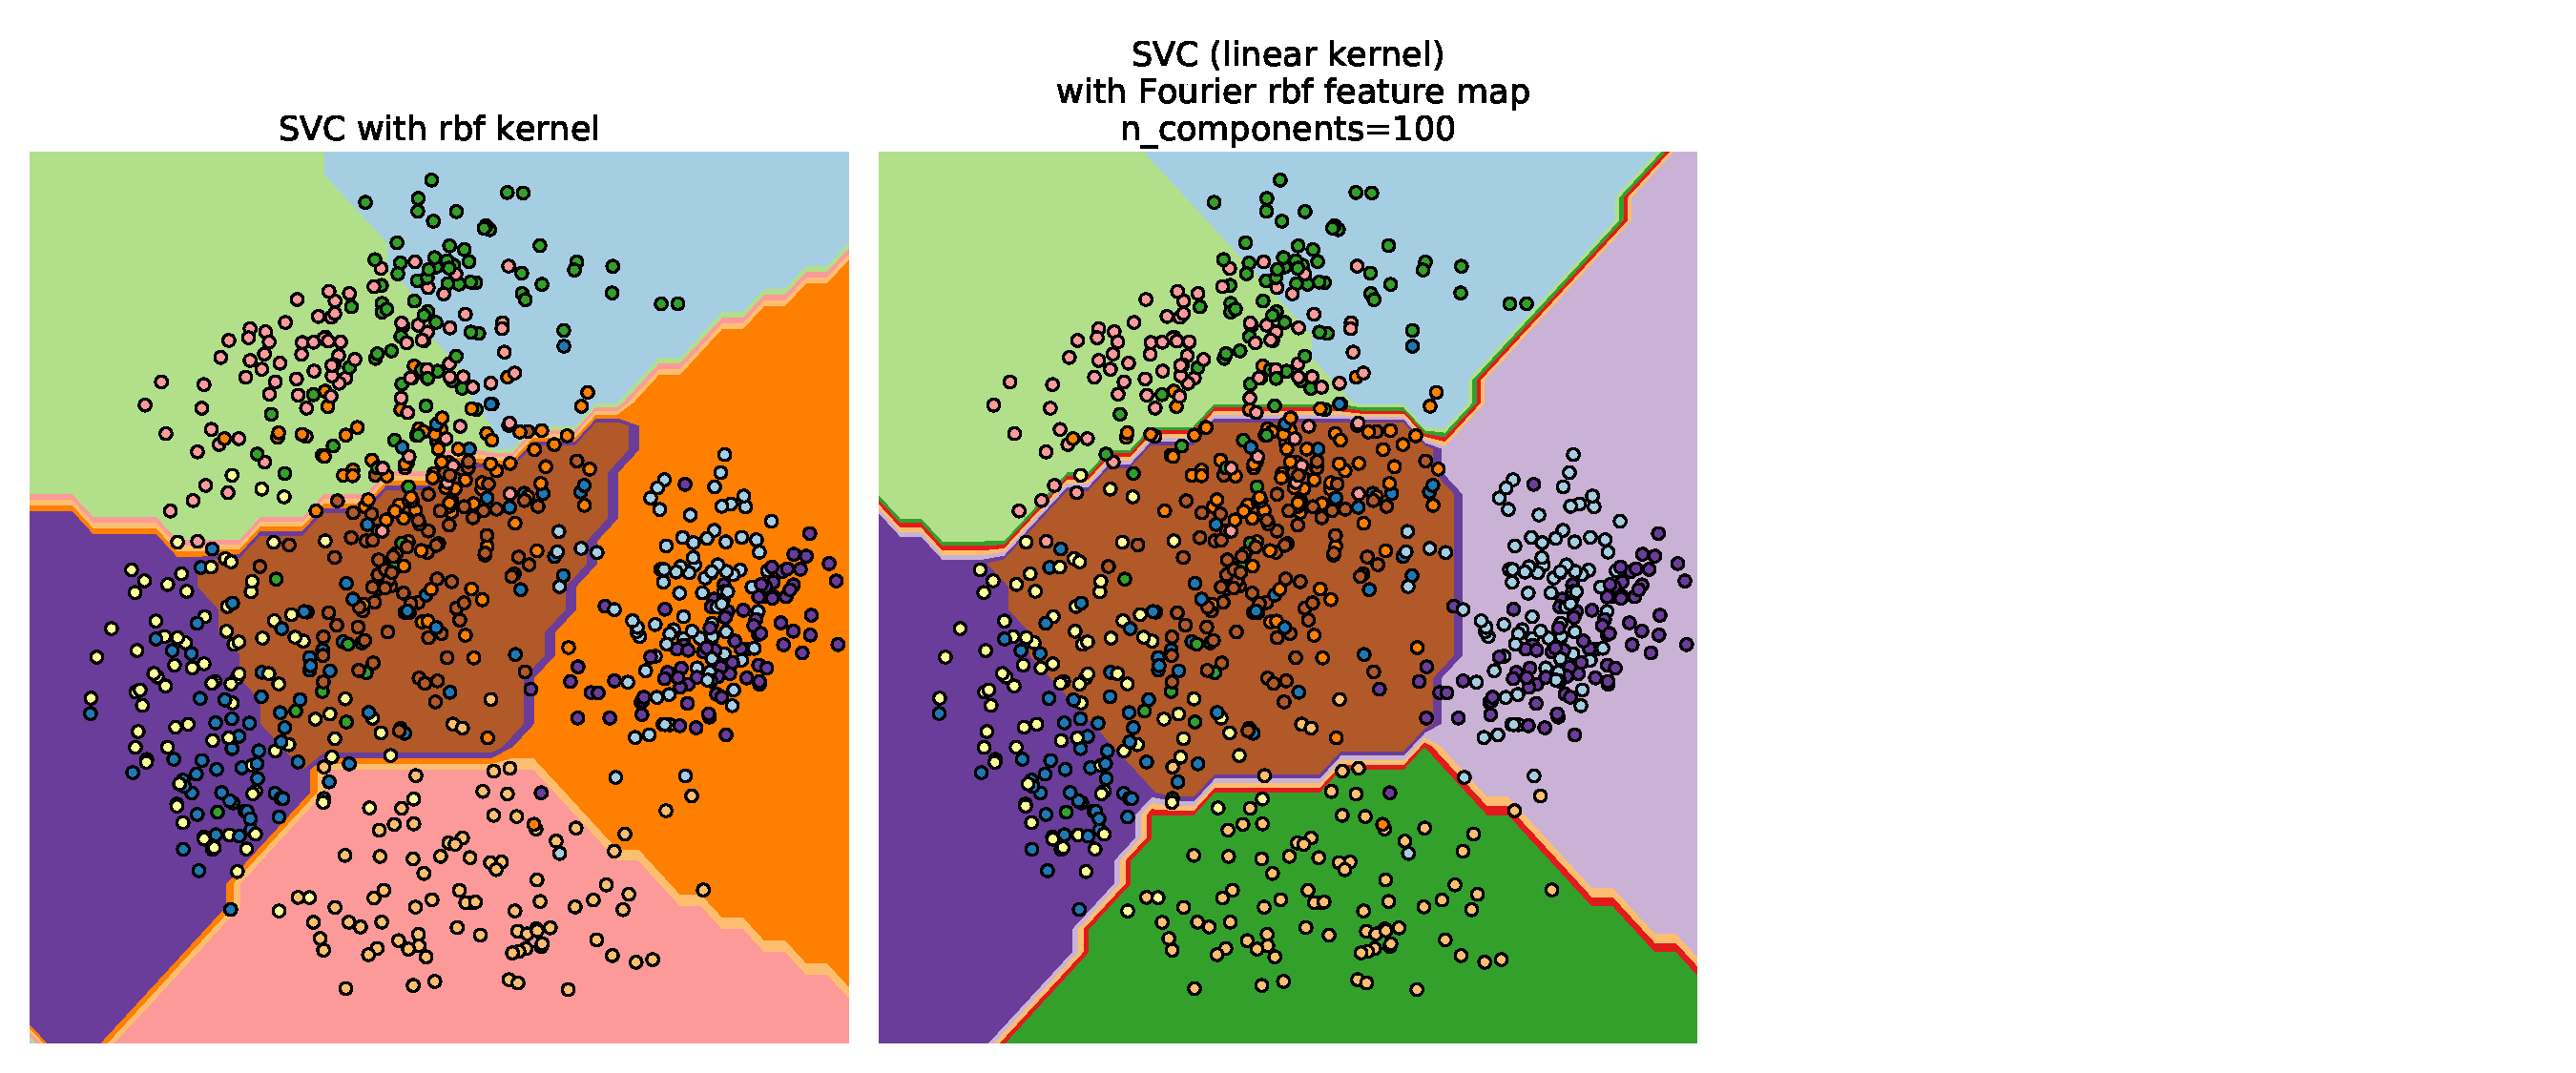
\includegraphics[scale=0.5]{images/frontiere.pdf}
    \caption{SVC (\textit{Support Vector Classification}) with two different methods.}
    \label{frontiere}
\end{figure}

Unlikely, I did not manage to code the Random binning features part. 

\newpage
\section{Conclusion}
We have presented randomized features whose inner products uniformly approximate many popular kernels, and demonstrated that these features are a powerful and economical tool for large-scale supervised learning.\\

We can note that any mixture of these features (like combining partitioning with Fourier features or sampling frequencies from mixture models) can be readily computed and applied to learning problems. 


\newpage
\bibliographystyle{alpha}
\nocite{*}
\bibliography{../biblio.bib}
\end{document}
